\chapter{Arkitektur}

%Her beskrives den overordnede systemarkitektur vha. en domænemodel efterfulgt af SysML/UML. Der tages stilling til hvilke dele af projektet, der skal realiseres i HW og hvilke der skal realiseres vha. SW. De vigtigste dele af arkitekturen beskrives for syste- mets HW og SW i en sådan grad, at læseren får det fornødne overblik over systemet. Der fokuseres på opdeling i blokke, moduler, pakker, klasser etc. Der fokuseres ligeledes på hvordan disse blokke/moduler/pakker/klasser kommunikerer indbyrdes, dvs. de overord- nede signaler/protokoller beskrives. For beskrivelse af detaljer angives reference til jeres ”arkitekturdokument” i projektets bilag.

\section*{Indledning} 
Dette kapitel har til formål at beskrive detekteringssystemets systemarkitektur. Gennem System Modeling Language (SysML) beskrives forholdet mellem de forskellige hardware- og softwareblokke samt, hvordan de internt kommunikerer med hinanden. Arkitekturen fungerer som en udviklingsramme for udviklingen af hardwaren og softwaren for  detekteringssystemet. 

Block definition diagram (BDD) og internal block diagram (IBD) for systemarkitekturen, samt sekvensdiagrammet for detekteringssystemets primære Use Case (Use Case 2) er beskrevet i dette kapitel. 

%System-, hardware- og softwarearkitektur er ydeligere beskrevet og dokumenteret i dokumentationens afsnit 4??. 

\section{Systemarkitektur}
\subsubsection{System BDD}

På Figur \ref{SystemBDD} ses det overordnede BDD for detekteringssystemet. BDD'et illustrerer hvilke hardware- og softwareblokke, som detekteringssystemet består af. Blokkene repræsenterer de forskellige hardware- og softwarekomponenter.   

\begin{figure}[H]
	\centering
	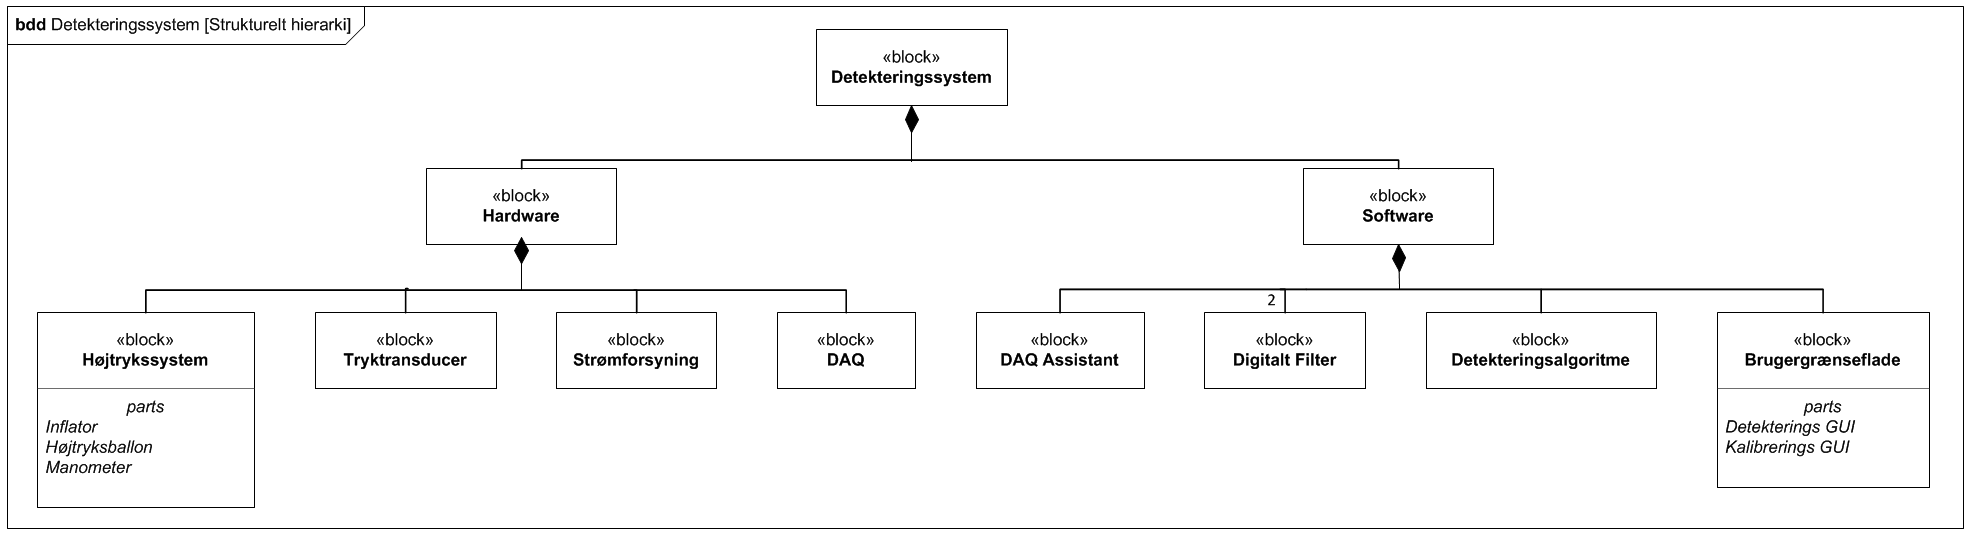
\includegraphics[width=1\textwidth]{Figure/SystemBDD}
	\caption{BDD for detekteringssystemet}
	\label{SystemBDD}
\end{figure}

I dokumentationen er BDD for hardware- og softwareblokkene med de ønskede egenskaber for komponenterne beskrevet. Se dokumentation afsnit 3.2.1 for hardware BDD og afsnit 3.3.1 for software BDD. 

\subsubsection{System IBD}
På Figur \ref{SystemIBD} ses det overordnede IBD for detekteringssystemet. IBD'et viser hele detekteringssystemets interne struktur. Det ses, hvordan de forskellige hardware- og softwareblokke intergerer med hinanden samt, hvilke in- og output signaler de enkelte blokke har. 

\begin{figure}[H]
	\centering
	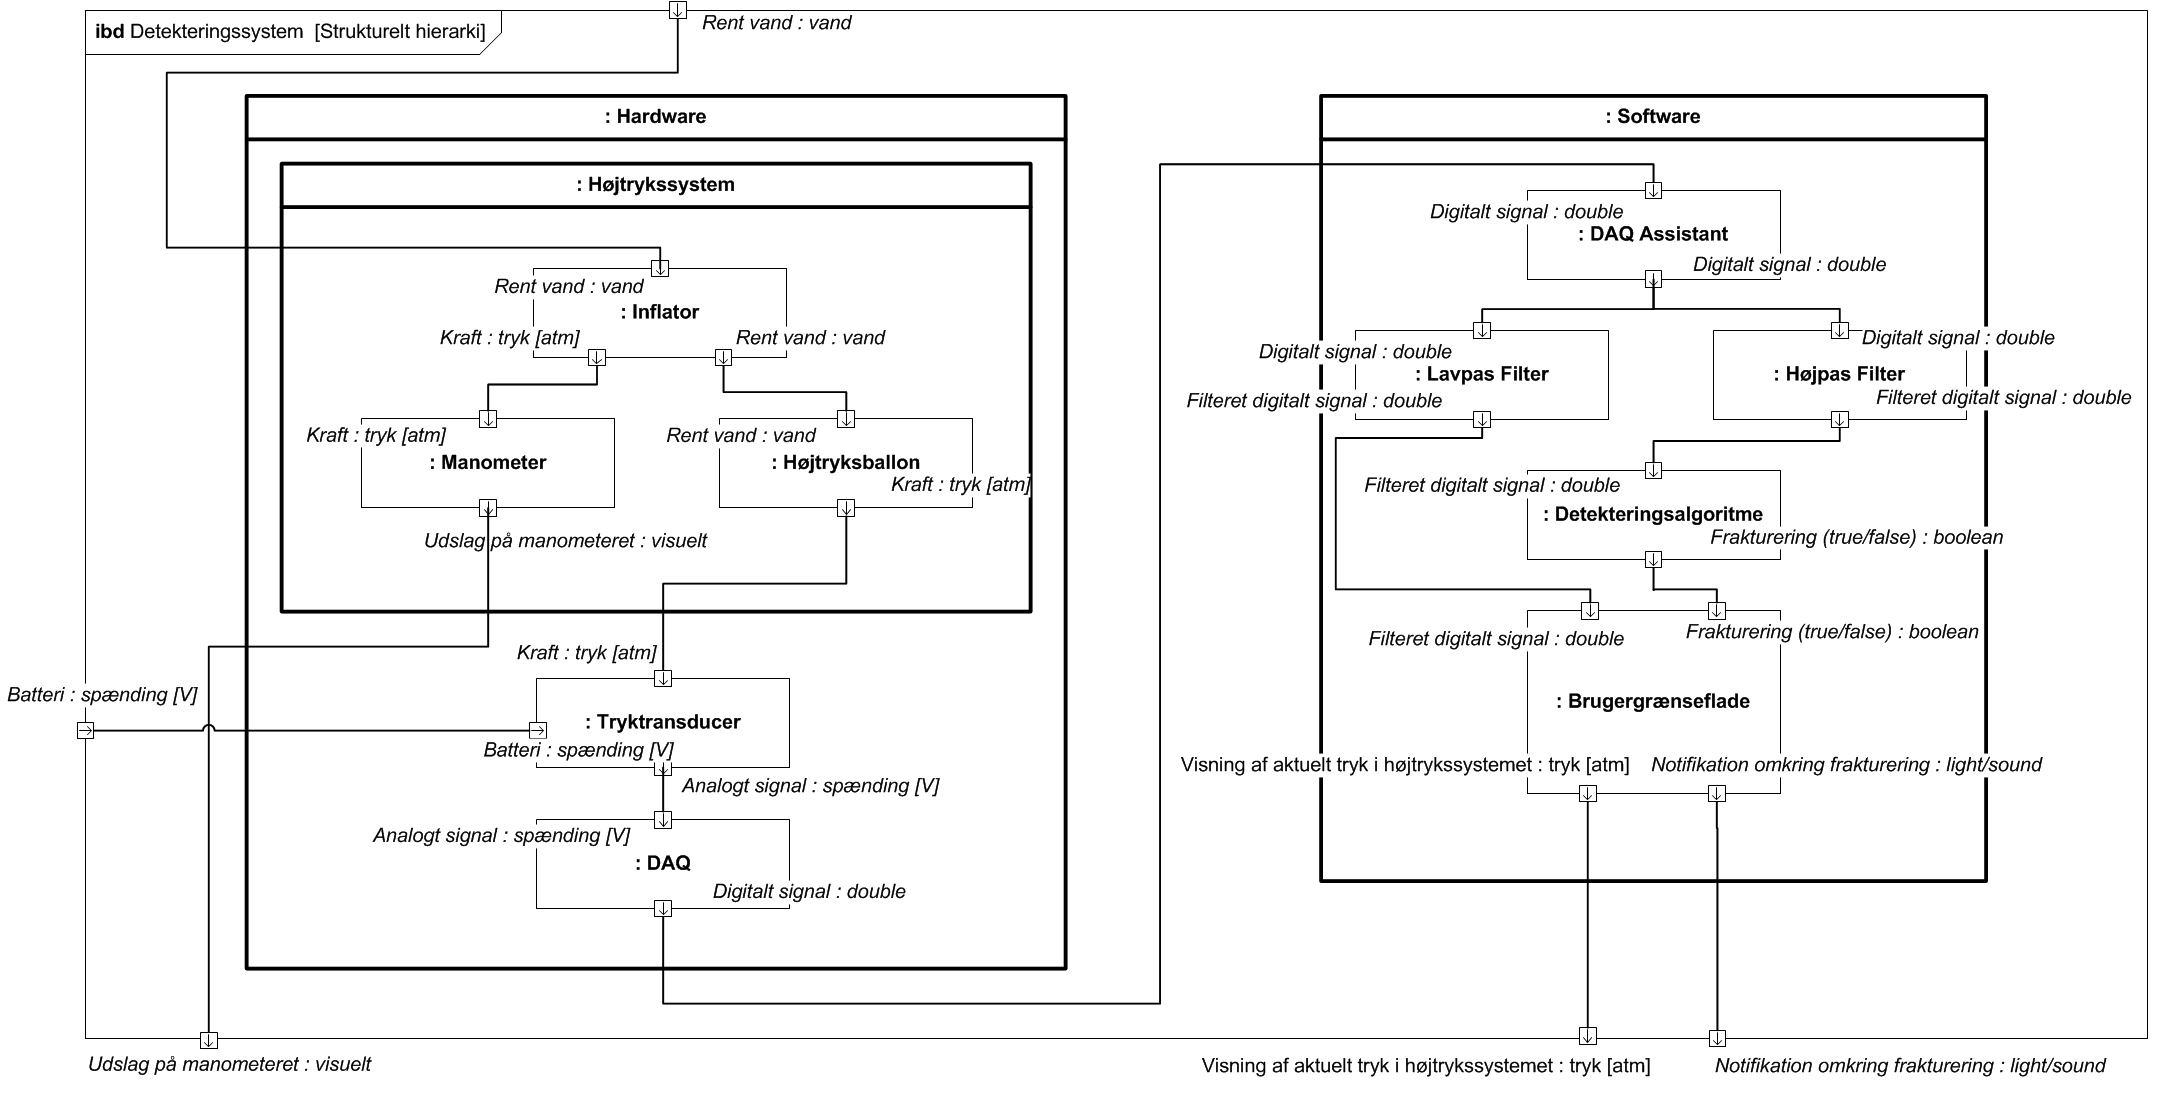
\includegraphics[width=1\textwidth]{Figure/SystemIBD}
	\caption{IBD for detekteringssystemet}
	\label{SystemIBD}
\end{figure}

I hardwareblokken fremgår det, at inflatoren fyldes med rent vand. Når operatøren påbegynder inflateringen genereres en kraft, udtrykt som et tryk målt i atmosfære [atm], der analogt vises på manometeret. Inflateringen medfører også, at højtryksballonen fyldes med det rene vand fra inflatoren, hvilket generer en udadgående kraft, udtrykt som et tryk målt i atm. Dette tryk måles af tryktransduceren, som konverterer det målte tryk til et analogt signal udtrykt som en spændning [V]. Tryktransduceren skal endvidere være tilkoblet en strømforsyning. I DAQ'en konverteres det analoge signal, udtrykt som en spænding [V], til et digitalt signal af typen double.

Det digitale signal kan nu indlæses af DAQ Assistant og anvendes i de resterende softwareblokke. Det digitale signal lavpasfiltreres for at sikre en mere stabil visning af det aktuelle tryk eller spænding på brugergrænsefladen. Det digitale signal højpasfiltreres inden det analyseres af detekteringsalgoritmen. Når detekteringsalgoritmen detekterer et transient trykfald ændres boolean-værdien til 'true' og en notifikation, udtrykt ved lyd og lys, forekommer på brugergrænsefladen.   

I dokumentationen er der lavet IBD for hardware- og softwareblokkene, som beskriver den interne kommunikation mellem komponenterne. Se dokumentation afsnit 3.2.2 for hardware IBD og afsnit 3.3.2 for software IBD.  

\subsubsection{Sekvensdiagram}
Et sekvensdiagram (SD) beskriver step-by-step forløbet for en specifik Use Case. Det består af boundary-klasser, som er de blokke, der intergerer med hinanden i den specifikke Use Case samt en controller-klasse, med navn efter Use Casen.

Detekteringssystemets funktionalitet er beskrevet gennem tre Use Cases, se afsnit \ref{usecasebeskrivelse}. Den primære Use Case er Use Case 2: Detektering, da det er her detekteringssystemets primære funktion udspilles. På Figur \ref{UC2SD} ses SD for Use Case 2.   

\begin{figure}[H]
	\centering
	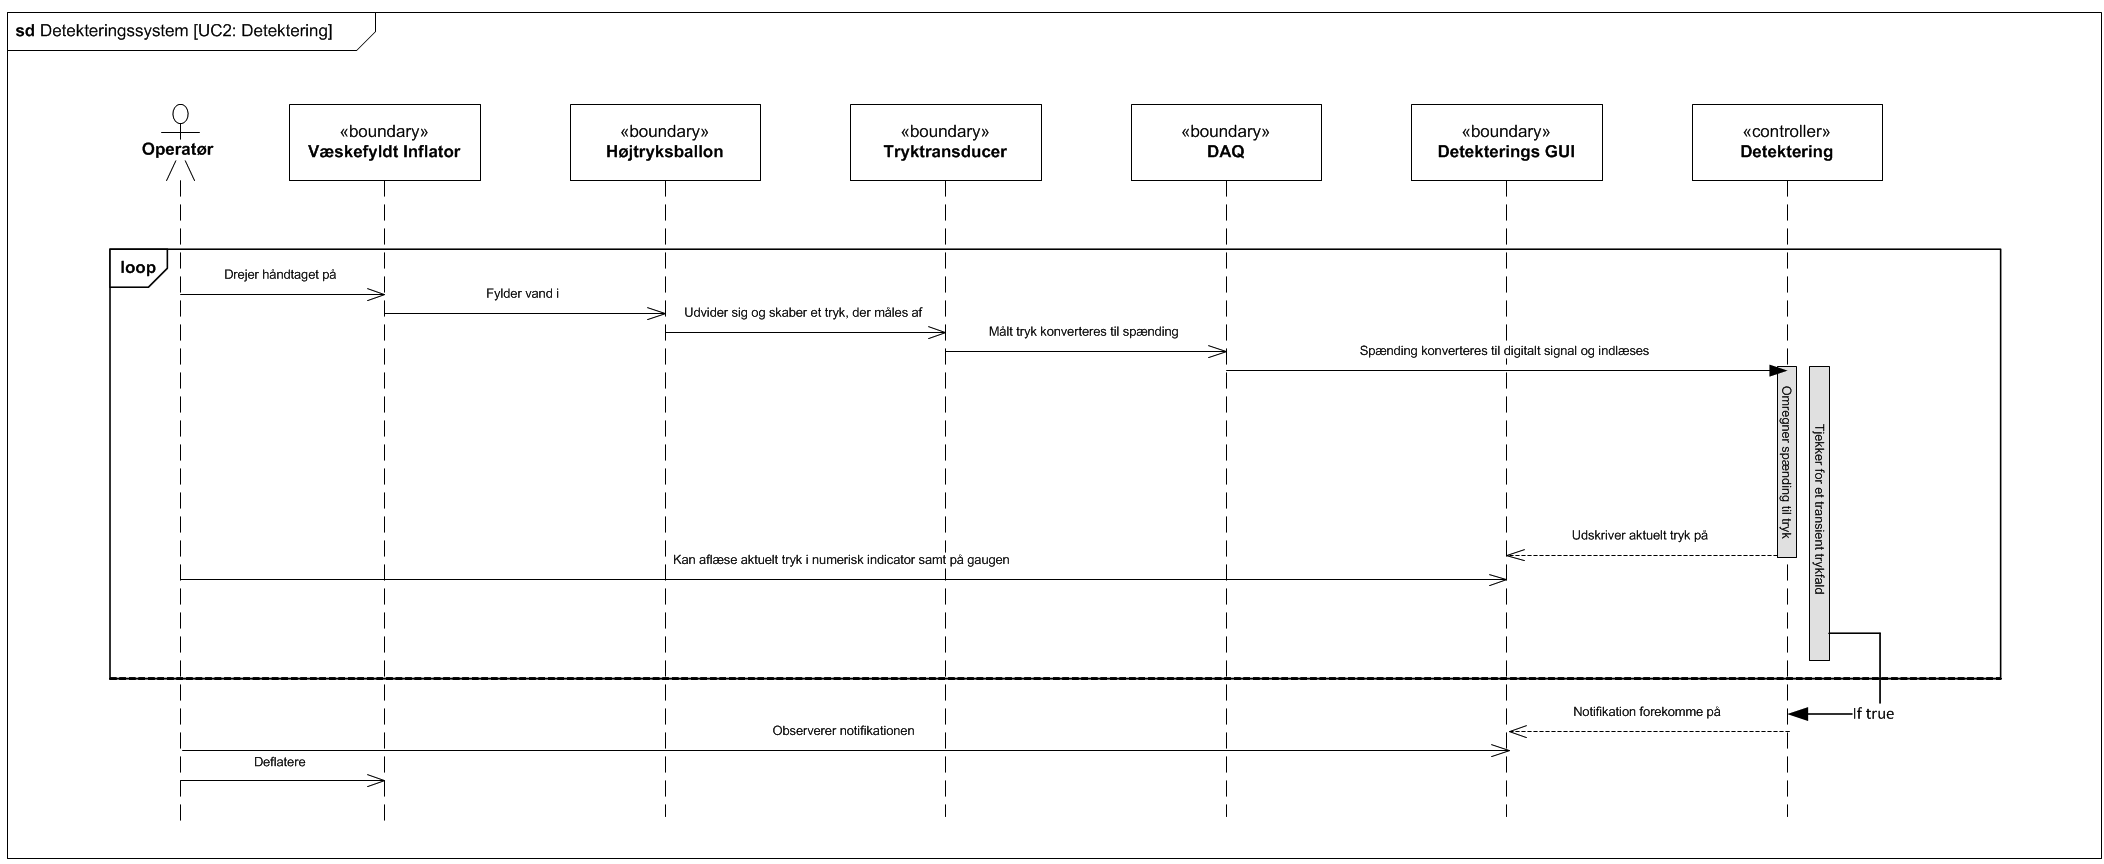
\includegraphics[width=1\textwidth]{Figure/UC2SD}
	\caption{SD for Use Case 2}
	\label{UC2SD}
\end{figure}  

Operatøren, som er den primære aktør i denne Use Case, drejer håndtaget på den væskefyldte inflator, hvilket medfører, at højtryksballonen bliver fyldt med vand. Højtryksballonen skaber en udadgående kraft, som måles af tryktransduceren. Tryktransduceren konverterer det målte tryk til en spænding. Denne spænding konverteres endvidere til et digitalt signal af DAQ’en. Det digitale signal indlæses af controlleren, hvor signalet bliver omregnet til det aktuelle tryk i højtryksballonen, hvilket bliver udskrevet på detekterings GUI’en. Alt dette foregår i et loop, hvor controlleren kontinuerligt tjekker for et transient trykfald. Dette loop afbrydes, når controlleren detekterer et transient trykfald, hvortil en notifikation vil forekomme på detekterings GUI’en. Efter et transient trykfald er detekteret, deflaterer operatøren inflatoren.

Se dokumentation afsnit 3.3.3 for grafisk tegning af Use Case 1 og afsnit 3.3.4 for SD af Use Case 3.  














